\FloatBarrier
\section{Systems Measurements and Applicability}
\label{app:systems}
The encoder cache moves document work from each query into preparation. We measure both sides of this exchange: full-source and same-evidence request costs, persistent storage and transfer, and the number of queries needed to amortize Write. Each timer below states which costs it includes.
\subsection{Local full-source comparison and depth diagnostics}
\label{app:local-infra}
\begin{figure}[htbp]
\centering
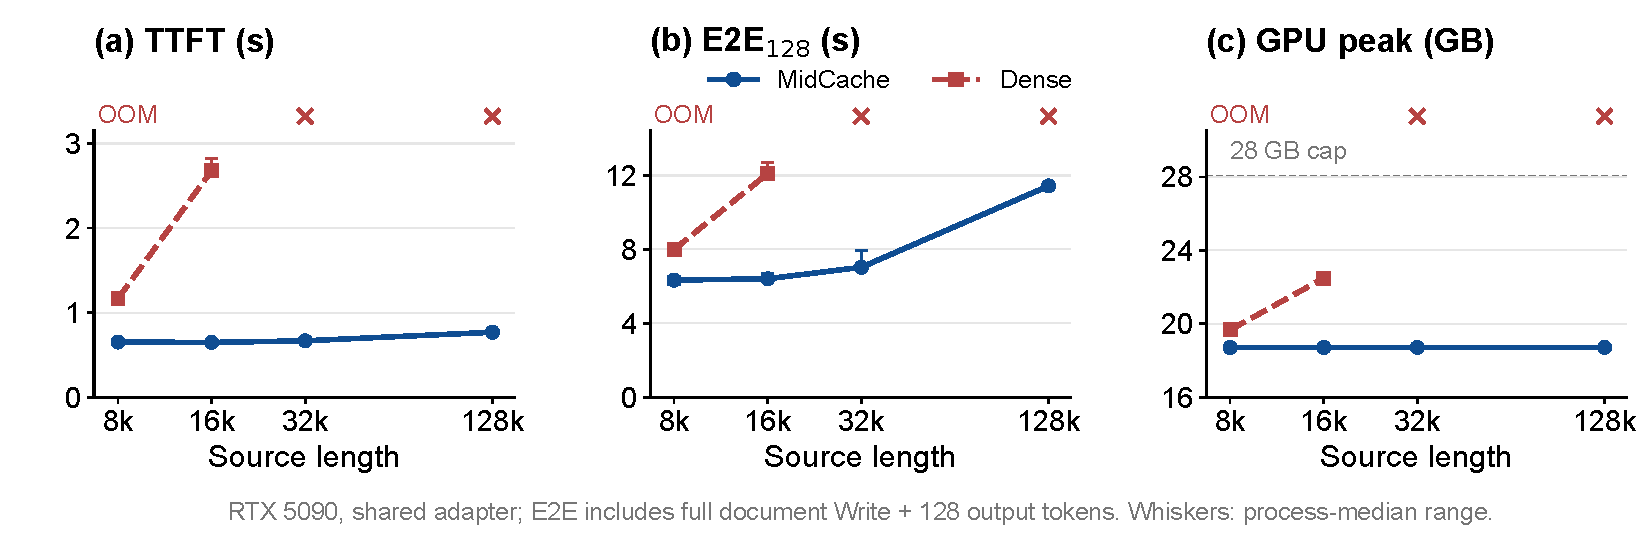
\includegraphics[width=\linewidth]{figures/source_scaling.pdf}
\caption{\textbf{Source-length scaling on RTX 5090.} These are the Table~\ref{tab:infra}(a) measurements with a shared adapter and three documents per length. Source length uses a base-two logarithmic axis. Latency markers are medians of three process medians; whiskers show their range, not a confidence interval. TTFT excludes document Write; E2E includes fresh document preparation and a fixed 128-token output. GPU values are maximum TTFT allocated peaks including weights. Red crosses above the axes mark Dense OOMs at 32k and 128k under the 28 GB allocator cap; they have no numerical ordinate. MidCache's 32k/128k measurements use a tighter 26 GB cap. Full inputs, repetition counts, and timing boundaries are specified in this appendix.}
\label{fig:source-scaling}
\end{figure}

The RTX 5090 measurements use Windows, PyTorch 2.7.1+cu128, Transformers 5.16.1, two intra-op and sixteen inter-op CPU threads, and SDPA with explicit KV-head repetition. Qwen3-8B weights remain bf16 and fully GPU resident. All local methods share the principal unmerged fp32 rank-32 suffix adapter spanning layers 12--35, with the training configuration specified in Appendix~\ref{app:protocol}. The PG-19 timing inputs differ from the benchmark questions, so these costs are not item-paired with Table~\ref{tab:accuracy}.

At each length, three saved PG19 documents supply the complete source and its next 512 tokens as the query: book indices 0/1/2 at 8k, 16k, and 32k, and 0/1/32 at 128k. Queries therefore differ across source lengths. These are fixed, unscored systems workloads. MidCache's iterative token-ID BM25 uses the first 32 query tokens, hop width two, and top-12 source-order chunks of 512 tokens. Its suffix receives 6,657 residual-state positions at $j=12$: 6,144 cached source positions, 512 query positions, and one BOS sink. Dense instead receives all 8,705, 16,897, 33,281, or 131,585 token IDs without retrieval.

\paragraph{Full-source Dense under the memory limit.}
\label{app:local-dense28}
\begin{table}[htbp]
\centering
\small
\setlength{\tabcolsep}{4pt}
\begin{tabularx}{\linewidth}{lll*{5}{>{\raggedleft\arraybackslash}X}}
\toprule
Source & Method & Phase & P1 & P2 & P3 & Peak GB & OOM\\
\midrule
8k & Dense & Prefill & 1194.4 & 1222.1 & 1159.5 & 19.66 & 0/9\\
 &  & TTFT & 1165.9 & 1231.9 & 1162.5 & 19.66 & 0/9\\
 &  & E2E$_{128}$ & 8124.3 & 7987.6 & 7643.4 & 19.66 & 0/9\\
\midrule
8k & CoMem & Prefill & 607.1 & 640.5 & 601.9 & 18.68 & 0/9\\
 &  & TTFT & 652.6 & 672.4 & 639.2 & 18.71 & 0/9\\
 &  & E2E$_{128}$ & 6537.7 & 6331.6 & 6073.1 & 18.71 & 0/9\\
\midrule
16k & Dense & Prefill & 2819.0 & 2684.8 & 2679.0 & 22.49 & 0/9\\
 &  & TTFT & 2820.0 & 2681.3 & 2680.2 & 22.49 & 0/9\\
 &  & E2E$_{128}$ & 12680.3 & 12085.8 & 12093.9 & 22.49 & 0/9\\
\midrule
16k & CoMem & Prefill & 634.3 & 606.5 & 602.8 & 18.68 & 0/9\\
 &  & TTFT & 685.2 & 647.0 & 648.0 & 18.71 & 0/9\\
 &  & E2E$_{128}$ & 6703.1 & 6407.2 & 6392.6 & 18.71 & 0/9\\
\midrule
32k & Dense & Prefill & OOM & OOM & OOM & OOM & 9/9\\
 &  & TTFT & OOM & OOM & OOM & OOM & 9/9\\
 &  & E2E$_{128}$ & OOM & OOM & OOM & OOM & 9/9\\
\midrule
128k & Dense & Prefill & OOM & OOM & OOM & OOM & 9/9\\
 &  & TTFT & OOM & OOM & OOM & OOM & 9/9\\
 &  & E2E$_{128}$ & OOM & OOM & OOM & OOM & 9/9\\
\bottomrule
\end{tabularx}
\caption{Fresh RTX 5090 measurements with the shared adapter and a 28 GB total CUDA allocator cap. Dense receives the full source plus 513 query/BOS tokens; CoMem resumes from cached $j=12$ residual states of 12 selected chunks. P1--P3 are independent process medians in milliseconds, each from three documents with one warmup and three formal repetitions per document. OOM counts failed document/process cells out of nine; repetitions stop after an OOM. Failed entries have no completed latency or peak-memory value. Peak GB is the maximum allocated memory including weights. Retained 32k/128k CoMem process results appear in the subsequent diagnostic tables.}
\label{tab:dense5090}
\end{table}

Dense uses the standard model forward with a complete KV cache and only the final vocabulary logits. There is no truncation, quantization, CPU weight/KV offload, or RoPE extension. Fused SDPA is required and the quadratic-memory math backend is disabled. A 28,000,000,000-byte process CUDA allocator cap includes weights, inputs, KV, and temporary tensors; both allocated and reserved memory remain within it. Desktop and driver-context overhead are separate from this allocator budget. Each of three fresh processes attempts every source length, document, and phase. A CUDA OOM is recorded with its error and full input shape; remaining repetitions of that failed cell are skipped. Other errors fail the worker rather than becoming OOM entries. Any failed prescribed document/process cell makes the corresponding overview entry OOM, without a latency or a selectively reported successful-subset mean.

Dense Prefill starts with the entire ID sequence on GPU and ends at first logits. TTFT starts with pretokenized CPU source/query, assembles and pins the full IDs, transfers them, and runs the same cached forward. E2E continues to 128 generated token IDs, including the first token and 127 cached decode steps; EOS does not shorten this fixed budget. Model loading, tokenization/detokenization, queues, network transport, and external I/O are excluded. Each worker checks cached greedy decoding against full recomputation before formal measurement; the short-source workers also check MidCache's cached decode against pack recomputation. Beyond-native full-source timings are not an accuracy claim.

\paragraph{MidCache preparation and request boundaries.}
At 8k and 16k, both methods are measured in the same three processes under the 28 GB cap, with shuffled method and phase order. At 32k and 128k, MidCache uses a stricter 26 GB allocator cap. The same model, adapter, and saved inputs are used within each source length. MidCache Prefill starts with GPU-ready residuals, while TTFT additionally includes BM25 construction/selection, pinned fetch, and sink/query Write. These two phases exclude document Write and decode. E2E begins with the pretokenized source/query and includes preparing a new pinned store, independently writing every source chunk, retrieval, fetch, sink/query Write, prefill, and a fixed 128-token output. It stops before store/cache teardown. Document Write is charged in full, without amortization. At 128k the residual store is 1 GiB of CPU memory, separate from GPU allocation.

Dense at every length and MidCache at 8k/16k use one warmup and three formal repetitions per successful cell: 27 formal observations per source/method/phase across three processes and three documents. MidCache Prefill and TTFT at 32k/128k use five warmups and twenty formal repetitions per document (180 observations per cell); MidCache E2E at these lengths uses one warmup and three repetitions (27 observations). Reported latencies are medians of process medians; GPU peaks are maximum allocated bytes including weights. Phases are timed independently, so small Prefill/TTFT median reversals can occur with run-to-run variation; their difference is not an isolated transfer-cost estimate. E2E is timed directly, not added from separate medians. All local inputs and generated IDs, phase boundaries, checks and raw attempts are saved.

\paragraph{Same-evidence depth diagnostics.}
\begin{table}[htbp]
\centering
\small
\setlength{\tabcolsep}{4pt}
\begin{tabular}{@{}lllrrrr@{}}
\toprule
Source & Method ($k$) & Phase & Process 1 & Process 2 & Process 3 & Peak GB\\
\midrule
32k & Replay (12) & Prefill & 835.1 & 836.3 & 835.0 & 19.01\\
32k & MidCache (12) & Prefill & 611.9 & 611.5 & 611.8 & 18.68\\
32k & Replay (12) & TTFT & 867.7 & 867.7 & 868.5 & 19.01\\
32k & MidCache (12) & TTFT & 667.5 & 666.7 & 667.6 & 18.71\\
\midrule
128k & Replay (12) & Prefill & 875.1 & 882.4 & 835.9 & 19.01\\
128k & MidCache (12) & Prefill & 638.8 & 620.3 & 616.6 & 18.68\\
128k & Replay (12) & TTFT & 972.1 & 1008.6 & 957.7 & 19.01\\
128k & MidCache (12) & TTFT & 768.6 & 796.5 & 760.1 & 18.71\\
\bottomrule
\end{tabular}
\caption{RTX 5090 same-evidence depth diagnostic, separate from full-source Dense. Each process latency is the median over three documents and twenty formal repetitions per document, in milliseconds. The MidCache main-table latency is the median of these process medians; memory is the maximum allocated peak over all 180 formal observations per source length, method, and phase. Both methods use the same top-12 selected pack of 6,657 tokens and the same principal adapter; this cost workload supplies no accuracy evidence.}
\label{tab:local-infra-processes}
\end{table}

\begin{table}[htbp]
\centering
\small
\setlength{\tabcolsep}{4pt}
\begin{tabular}{@{}llrrrrr@{}}
\toprule
Source & Method & Process 1 & Process 2 & Process 3 & E2E$_{128}$ & Peak GB\\
\midrule
32k & Raw replay & 6810.1 & 6504.1 & 7127.9 & 6810.1 & 19.01\\
32k & CoMem & 7021.3 & 7026.1 & 7938.1 & 7026.1 & 18.71\\
128k & Raw replay & 6835.7 & 6916.4 & 6684.6 & 6835.7 & 19.01\\
128k & CoMem & 11426.8 & 11491.2 & 11241.1 & 11426.8 & 18.71\\
\bottomrule
\end{tabular}
\caption{RTX 5090 same-evidence E2E diagnostic, distinct from full-source Dense, including document preparation and a fixed 128-token output. Times are milliseconds. Each process median covers three documents and three formal requests per document after one warmup; E2E is the median across three independent processes (27 requests per row). Full-request GPU peaks are separate from the Prefill/TTFT peaks in Table~\ref{tab:infra}.}
\label{tab:local-e2e}
\end{table}

The raw-replay depth measurements send the same top-12 selected tokens through all layers ($j=0$), using MidCache's adapter, evidence, order, and sink. They are depth diagnostics, separate from the full-source Dense baseline in Table~\ref{tab:infra}. Their GPU inputs remain 6,657 tokens at both source lengths. Three-process Prefill/TTFT and E2E observations use the respective repetition counts above. The E2E diagnostic includes source preparation and fixed-length generation, with a fresh full-document residual store for MidCache; it does not describe Dense on the entire source.

The H20 matched-depth and TTFT-calibration experiments do not measure GPU peaks; the RTX 5090 experiments report device-specific memory costs. Persistent-store capacity, online request peak allocation, and document-Write peak allocation remain separate quantities.

\subsection{B300 full-context and selected-pack comparison}
\label{app:b300-recheck}
\begin{table}[htbp]
\centering
\small
\setlength{\tabcolsep}{7pt}
\begin{tabular}{@{}lllrr@{}}
\toprule
Method & Adapter & Model tokens & Latency (ms) & Peak GPU (GB)\\
\midrule
\multicolumn{5}{l}{\textit{GPU-ready prefill to first logits}}\\
Dense & Off & 131,585 & 14,634.5 & 50.17\\
Dense & Shared & 131,585 & 15,919.1 & 62.03\\
Raw replay & Shared & 6,657 & 246.4 & 19.04\\
CoMem & Shared & 6,657 & 194.8 & 18.71\\
\midrule
\multicolumn{5}{l}{\textit{Selected-pack TTFT with online selection and fetch}}\\
Raw replay & Shared & 6,657 & 428.9 & 19.04\\
CoMem & Shared & 6,657 & 387.9 & 18.74\\
\bottomrule
\end{tabular}
\caption{B300 measurements on three fixed 128k-source PG19 workloads. Each latency is the median of three independent process medians, each over three documents and three formal repeats after one warmup. Peak GPU allocation is the maximum over all 27 formal repetitions per row, including weights. Only the full-context diagnostic disables LoRA; all principal comparisons share the same adapter. Source length, selected-pack length, and timer boundary are distinct.}
\label{tab:b300-recheck}
\end{table}

The B300 experiment uses the same source/query tokens, selected chunk IDs, backbone, and unmerged fp32 adapter as the local 128k supplement. One Slurm-allocated B300 reports CUDA compute capability 10.3 and 287.4 GB total device memory; its driver display name is L20D. Software is PyTorch 2.14.0+cu130, Transformers 5.16.1, and PEFT 0.20.0, with two intra-op and four inter-op CPU threads. Native GQA uses fused SDPA; the math attention backend is disabled. Model weights remain bf16 and fully GPU resident.

Dense processes BOS, the complete 131,072-token source, and the 512-token query: 131,585 input tokens. It constructs a full KV cache and projects only the final vocabulary logits. MidCache and raw replay use the same 6,657-token selected pack. All document chunks are written into CPU-pinned memory before the timer; Read begins with GPU-ready tensors. TTFT additionally includes CPU iterative BM25 (including its term-frequency construction), fetch, and sink/query Write. Neither timer includes document Write, tokenization, decode, or external I/O. Source/query inputs are unscored and unextended; these costs do not establish accuracy beyond the native position window.

The same-adapter full-context/MidCache Read ratio is $81.7\times$, but the same-pack depth-only ratio is $1.265\times$ and the selected-pack TTFT ratio is $1.105\times$. The large full-context ratio therefore combines selection with depth reuse. The stock, adapter-disabled dense diagnostic gives $75.1\times$ against MidCache. Each process checks the loaded $j=0$ reader against stock last-position logits on a 256-token input before timing.

\subsection{Write-once serving and store placement}
\begin{table}[htbp]
\centering
\small
\setlength{\tabcolsep}{4pt}
\begin{tabular}{@{}lrrrr@{}}
\toprule
Source / store & $G=1$ & $G=32$ & $G=128$ & $G=512$ \\
\midrule
32k / CPU pinned & 8.9 & 9.2 & 10.9 & 94.0 \\
32k / GPU resident & 8.4 & 7.7 & 5.5 & $\infty$ \\
128k / CPU pinned & 27.6 & 29.7 & 37.4 & 520.1 \\
128k / GPU resident & 25.8 & 26.8 & 27.2 & 164.2 \\
1M / CPU pinned & 198.2 & 266.7 & 421.3 & 302.6 \\
1M / GPU resident & 180.2 & 183.0 & 190.6 & 574.7 \\
\bottomrule
\end{tabular}
\caption{Full repeated-query break-even grid. Each cell is $Q^\star$ in queries from Equation~\ref{eq:breakeven}; $G$ is generated tokens. Fetch, Read, and decode are included. Infinite crossover denotes nonpositive measured per-query savings. Values derive from three process medians and are workload-specific.}
\label{tab:break-even}
\end{table}

The serving grid compares matched selection, examples, and packs. Per-query time includes fetch, model Read, and decode; common selection cancels from Equation~\ref{eq:breakeven}. It assumes a stable, fully prepared source store: every selected chunk is a cache hit, with no eviction or corpus update charged between queries. Thus $Q^\star$ describes reuse of that store rather than an observed application hit rate. The 32k CPU-pinned preparation is 2.253\,s, compared with 2.16\,ms for the raw-token index. Values are derived from three process medians. The large-output crossovers are sensitive to small differences in decode time and should not be interpreted as a monotonic scaling law. In particular, a finite crossover is absent in one 32k GPU-resident cell.

\begin{table}[htbp]
\centering
\small
\setlength{\tabcolsep}{4pt}
\begin{tabular}{@{}lrrrrl@{}}
\toprule
Backend & Write GB/s & Fetch ms & H2D ms & Peak QPS & Outcome \\
\midrule
GPU resident & OOM & --- & --- & --- & 128 GiB $>$ 95 GiB \\
CPU pinned & 139.6 & 0.81 & 1.41 & 941 & 235 GB host \\
Local NVMe & 2.45 & 13.42 & 0.91 & 264 & 2.18 GB host \\
Network / CEPH & 1.66 & 79.20 & 1.20 & 42 & 2.19 GB host \\
\bottomrule
\end{tabular}
\caption{Persistent-store microbenchmark at 16M tokens. The same 50.3 MB top-12 pack is fetched per query; medians use seven repetitions after two warmups. Peak QPS selects the best of 1/4/16 clients and excludes model inference and retrieval.}
\label{tab:store-tiers}
\end{table}

The storage microbenchmark uses a 16M-token residual store of 128 GiB and fetches a fixed 50.3\,MB pack per query. Medians use seven repetitions after two warmups; peak QPS is the best of 1, 4, and 16 concurrent clients. These measurements include storage and transfer only, excluding BM25 and model inference. GPU residence fits 8M tokens at 64.98\,GB peak but not 16M. Off-GPU storage preserves bounded transfer volume while adding tier-dependent latency. Its QPS is not end-to-end serving throughput.

\subsection{Model timing and full-prefill references}
\begin{table}[htbp]
\centering
\small
\setlength{\tabcolsep}{4pt}
\begin{tabular}{@{}lrrrrr@{}}
\toprule
Length & Full s & CoMem s & Ratio & Full GB & CoMem GB \\
\midrule
8k & .165 & .309 & .53 & 19.92 & 17.60 \\
16k & .356 & .441 & .81 & 24.55 & 17.67 \\
32k & .826 & .681 & 1.21 & 33.82 & 17.79 \\
64k & 2.104 & 1.200 & 1.75 & 52.34 & 18.04 \\
128k & 6.035 & 2.202 & 2.74 & 89.39 & 18.54 \\
\bottomrule
\end{tabular}
\caption{Same-adapter Write-inclusive pipeline on one B200. Ratio is full time divided by CoMem time. Full processes the entire source; CoMem includes document Write, CPU retrieval, query Write, and upper-layer Read. Index construction and external I/O are excluded. Memory is peak GPU allocation.}
\label{tab:pipeline-lengths}
\end{table}

The same-adapter B200 pipeline includes document Write, CPU retrieval, query Write, and upper-layer Read through first logits, but excludes BM25 index construction and external I/O. Software is bf16/SDPA with PyTorch 2.10 and Transformers 5.5.4, and results are medians of three. Cached decode uses 20 greedy steps.

\begin{table}[htbp]
\centering
\small
\setlength{\tabcolsep}{4pt}
\begin{tabular}{@{}lrrrrr@{}}
\toprule
Method & Native A & Single 64/128k & MK 64/128k & VT 64/128k & LoCoMo F1/acc \\
\midrule
MidCache & 97.05 & 99/100 & 91/93 & 99.0/95.8 & 9.15/23.36 \\
SnapKV & 72.33$^\dagger$ & 100/100 & 94/91 & 80.0/84.8 & 9.21/22.05 \\
PyramidKV & 72.32$^\dagger$ & 100/100 & 93/89 & 88.6/86.8 & 9.13/22.10 \\
\bottomrule
\end{tabular}
\caption{Retained-KV quality at an approximately 6,657-token budget. SnapKV/PyramidKV long-length columns use full-prompt factor-4 YaRN; MidCache reads selected evidence without YaRN. $^\dagger$Native means include left-truncated 64k/128k inputs; both compression methods score 99.96 on 8k--32k. Cohort A and lexical LoCoMo metrics are used.}
\label{tab:kv-quality}
\end{table}

\begin{table}[htbp]
\centering
\small
\setlength{\tabcolsep}{4pt}
\begin{tabular}{@{}llrrr@{}}
\toprule
Method & Length & Full prefill ms & Peak GB & Decode ms/token \\
\midrule
SnapKV & 8k & 1,213 & 18.6 & 24.7 \\
SnapKV & 32k & 6,342 & 25.7 & 24.6 \\
SnapKV & 128k & 51,520 & 54.3 & 24.7 \\
PyramidKV & 8k & 1,203 & 18.6 & 24.7 \\
PyramidKV & 32k & 6,301 & 25.7 & 26.7 \\
PyramidKV & 128k & 51,520 & 54.3 & 26.8 \\
\bottomrule
\end{tabular}
\caption{Full-prefill retained-KV timing on H20, median of three with compression and 64-token generation. These methods prefill the whole source before eviction. The hardware differs from the B200 MidCache pipeline, so no cross-table speedup is inferred.}
\label{tab:kv-timing}
\end{table}

SnapKV and PyramidKV retain approximately the same token/KV budget but must first prefill the entire prompt. Their native 15-cell RULER means include left-truncated 64k/128k inputs, whereas both reach 99.96 on 8k--32k. The full-prompt long-length columns use factor-4 YaRN. The systems table times full prefill, compression, and a 64-token decode; the displayed decode column is per-token latency. These H20 values must not be combined with the B200 MidCache times to form a cross-table speedup.

\subsection{Same-backbone chunk-KV diagnostic}
\label{app:chunkkv}
\begin{table}[htbp]
\centering
\small
\setlength{\tabcolsep}{3.2pt}
\begin{tabular}{@{}llrrrrrr@{}}
\toprule
& Suffix & \multicolumn{4}{c}{LongEval accuracy} & Qasper & Payload \\
\cmidrule(lr){3-6}
Method & adapter & 8k & 16k & 32k & Mean & F1 & KiB/token \\
\midrule
Replay & off & 85 & 83 & 85 & 84.33 & 6.98 & .008 \\
Chunk-KV & off & 73 & 75 & 71 & 73.00 & 4.88 & 144 \\
MidCache (without LoRA) & off & 0 & 0 & 0 & 0.00 & 10.45 & 8 \\
\midrule
Replay & on & 80 & 77 & 76 & 77.67 & 4.65 & .008 \\
Chunk-KV & on & 59 & 62 & 46 & 55.67 & 3.68 & 144 \\
MidCache & on & 71 & 74 & 73 & 72.67 & 11.37 & 8 \\
\bottomrule
\end{tabular}
\caption{Matched evidence and explicit adapter control: 500 samples and 3,000 predictions, with 100 examples per LongEval length and all 200 Qasper examples. Both MidCache configurations use $j=12$ and $w=0$. Each path is evaluated with the same principal suffix adapter enabled or disabled; the adapter is trained for MidCache, not separately for the other paths. Chunk-KV is a CacheBlend-style reference with the first two layers fully recomputed and a fixed 15\% context-token set recomputed above them. Payload excludes the retrieval index and request-local KV; replay stores int64 IDs. These are quality measurements, not native-system latency comparisons.}
\label{tab:chunkkv}
\end{table}

The control uses the same 500 examples as Appendix~\ref{app:overlap-confirmation}: LongEval 8k/16k/32k with 100 examples per length and all 200 Qasper questions. Replay, MidCache at $j=12,w=0$, and the chunk-KV path share token IDs, selected chunks, order, sink 151643, and output budgets. Each runs with the principal adapter enabled and disabled, yielding 3,000 saved predictions across four B300 workers. An independent CPU pass checks scores, support, and selected IDs. The adapted replay and MidCache outputs match the corresponding overlap-control predictions exactly on all 500 examples.

The chunk-KV path independently prefills every selected chunk through all 36 layers, then reindexes its post-RoPE keys to contiguous pack positions. It fully recomputes layers zero and one of the assembled pack and ranks context positions by the squared L2 deviation of both keys and values at layer one. Layer-zero projections precede contextual attention and cannot supply this signal. The largest $\lceil .15N_{\mathrm{ctx}}\rceil$ deviations define a fixed source-token set recomputed through the remaining layers; sink and query positions are always recomputed. Thus the source token--layer fraction is approximately $(2+34\times.15)/36=19.72\%$, not 15\% of total execution. Full recomputation recovers stock last-position logits and the next three decode decisions in the GPU checks. This CacheBlend-style control does not implement gradual filtering, asynchronous fetch/compute overlap, or the native cache manager \citep{cacheblend}.

Table~\ref{tab:chunkkv} shows why adapter matching and deployment choice must both be visible. Applying the MidCache-trained adapter helps its own LongEval interface (0 to 72.67), but lowers replay from 84.33 to 77.67 and chunk-KV from 73.00 to 55.67. With the adapter shared, MidCache exceeds chunk-KV by 17.00 points ($[9.67,24.33]$ paired 95\% interval). Yet its 72.67 is close to unadapted chunk-KV's 73.00, so the shared-adapter difference is not evidence of an intrinsic 17-point advantage over reusable KV. No method-specific KV adapter is trained here.

On Qasper, MidCache scores 11.37 versus 4.88 for unadapted chunk-KV and 3.68 for adapted chunk-KV; all are low under the explicit-BOS, capped plain-text protocol. The shared-adapter Qasper difference is 7.68 points ($[6.30,9.07]$). Intervals use 10,000 paired resamples: examples within each LongEval length, or source-document clusters for Qasper. Full-depth bf16 GQA KV requires $2\times36\times8\times128\times2=147{,}456$ bytes/token, versus 8,192 for the residual. This establishes an 18-fold payload ratio; the quality control does not measure a native-system latency advantage.

\paragraph{Preparation, online latency, and storage.}
\begin{table}[p]
\centering
\footnotesize
\setlength{\tabcolsep}{3pt}
\begin{tabular}{@{}llrrrrrr@{}}
\toprule
Method & Adapter & Prep. & TTFT & Online$_{128}$ & E2E$_{128}$ & Store & GPU \\
 & & (ms) & (ms) & (s) & (s) & (MiB) & (GB) \\
\midrule
\multicolumn{8}{@{}l}{\textit{LongEval 8k ($n=5$)}} \\
Replay & off & 0.4 & 651.1 & 5.432 & 5.432 & 0.06 & 18.32 \\
Chunk-KV & off & 1174.2 & 352.8 & 5.109 & 6.291 & 1152.00 & 19.46 \\
CoMem (without LoRA) & off & 329.7 & 450.4 & 4.717 & 5.049 & 64.00 & 18.02 \\
\addlinespace[2pt]
Replay & on & 0.4 & 798.2 & 6.416 & 6.416 & 0.06 & 18.89 \\
Chunk-KV & on & 1441.6 & 393.9 & 5.995 & 7.445 & 1152.00 & 19.46 \\
CoMem & on & 328.1 & 597.9 & 5.688 & 6.015 & 64.00 & 18.59 \\
\midrule
\multicolumn{8}{@{}l}{\textit{LongEval 16k ($n=5$)}} \\
Replay & off & 0.6 & 658.3 & 5.437 & 5.438 & 0.12 & 18.33 \\
Chunk-KV & off & 2377.4 & 366.1 & 5.150 & 7.505 & 2304.00 & 19.46 \\
CoMem (without LoRA) & off & 664.2 & 457.9 & 4.711 & 5.379 & 128.00 & 18.02 \\
\addlinespace[2pt]
Replay & on & 0.6 & 811.1 & 6.426 & 6.427 & 0.12 & 18.90 \\
Chunk-KV & on & 2951.1 & 403.1 & 6.363 & 9.279 & 2304.00 & 19.46 \\
CoMem & on & 666.2 & 615.1 & 5.691 & 6.359 & 128.00 & 18.59 \\
\midrule
\multicolumn{8}{@{}l}{\textit{LongEval 32k ($n=5$)}} \\
Replay & off & 1.1 & 652.6 & 5.391 & 5.393 & 0.25 & 18.34 \\
Chunk-KV & off & 4647.1 & 364.4 & 5.094 & 9.739 & 4608.00 & 19.49 \\
CoMem (without LoRA) & off & 1311.2 & 457.0 & 4.703 & 6.023 & 256.00 & 18.04 \\
\addlinespace[2pt]
Replay & on & 1.1 & 803.7 & 6.399 & 6.400 & 0.25 & 18.92 \\
Chunk-KV & on & 5708.5 & 399.9 & 5.973 & 11.694 & 4608.00 & 19.49 \\
CoMem & on & 1319.2 & 613.2 & 5.685 & 7.012 & 256.00 & 18.62 \\
\midrule
\multicolumn{8}{@{}l}{\textit{Qasper ($n=5$)}} \\
Replay & off & 0.3 & 401.7 & 4.246 & 4.246 & 0.03 & 17.85 \\
Chunk-KV & off & 519.2 & 267.7 & 4.084 & 4.603 & 504.00 & 18.66 \\
CoMem (without LoRA) & off & 145.4 & 297.0 & 3.945 & 4.096 & 28.00 & 17.65 \\
\addlinespace[2pt]
Replay & on & 0.3 & 497.2 & 5.257 & 5.257 & 0.03 & 18.26 \\
Chunk-KV & on & 631.4 & 310.9 & 5.155 & 5.782 & 504.00 & 18.66 \\
CoMem & on & 146.5 & 389.9 & 5.190 & 5.334 & 28.00 & 18.06 \\
\bottomrule
\end{tabular}
\caption{Matched evidence costs on RTX 5090: 1,080 formal measurements over 20 prespecified examples, six method--adapter settings, three fresh processes, and three repetitions. Each cell reports the median of three process medians; each process median pools five examples and three repetitions. Preparation constructs a fresh whole-document pinned-CPU store. TTFT and Online start after preparation, include selection and fetch, and end at the first and 128th generated token, respectively. E2E is measured directly from preparation through token 128. Store is the median persistent payload, separate from peak GPU allocation including weights; all attempts fit the 28 GB allocator cap. CoMem uses $j=12,w=0$; replay processes the same selected evidence, not the full source. Chunk-KV is a synchronous CacheBlend-style reference. The 500-example quality evaluation is reported separately in Table~\ref{tab:chunkkv}.}
\label{tab:chunkkv-cost}
\end{table}

Table~\ref{tab:chunkkv-cost} uses the first five prespecified examples per task/length, the local software configuration above, and a 28 GB allocator cap. All 1,080 formal trials and 360 warmups complete, with method--adapter order shuffled in each process. Full-recomputation and query-placeholder checks pass: recomputing every query position makes zero-initialized query KV equivalent to independently cached query states at first logits. Generated IDs match across repetitions and processes within each setting.

Each trial freshly prepares the entire pretokenized document in pinned CPU memory: int64 IDs for replay, bf16 residuals for MidCache, or bf16 all-layer KV for chunk-KV. Preparation includes partitioning, pinning, and document Write. TTFT then includes BM25 construction/selection, transfer, sink/query handling, and inference through token one. Online continues to token 128 regardless of EOS; E2E directly times preparation through token 128, before teardown. Loading, tokenization/detokenization, external I/O, and scoring are excluded. Payload excludes selector metadata and transient raw IDs; GPU peaks include weights and preparation/inference allocations. Qasper lengths vary, so payload is a median. Separate medians need not add.

Chunk-KV has lower TTFT than MidCache in every cell under both adapter conditions, but needs more storage and preparation. At 32k with the shared adapter, chunk-KV versus MidCache takes 399.9 versus 613.2\,ms TTFT, 5.708 versus 1.319\,s preparation, and 11.694 versus 7.012\,s E2E. Process-median TTFT ranges are 397.4--412.8 and 608.2--640.0\,ms; these are descriptive, not confidence intervals. Persistent payload is 4,608 versus 256 MiB, while peak GPU allocation is 19.49 versus 18.62 GB: the 18-fold storage ratio does not describe GPU peaks. MidCache also has higher cold-request E2E than shared-adapter replay at 32k (7.012 versus 6.400\,s). These subset timings do not establish native CacheBlend performance or accuracy rankings.

\subsection{Latency-calibrated budget comparison}
\label{app:equal}
\begin{table}[htbp]
\centering
\small
\setlength{\tabcolsep}{4pt}
\begin{tabular}{@{}lcccc@{}}
\toprule
Replay selector & Replay / MidCache & Delta & Hierarchical CI & LOCO range \\
\midrule
Iterative BM25 & 64.78 / 53.22 & -11.56 & [-18.67, -5.11] & [-13.13, -9.50] \\
Frozen BGE & 54.22 / 53.22 & -1.00 & [-10.67, 8.33] & [-3.50, 1.75] \\
\bottomrule
\end{tabular}
\caption{Comparison at latency-calibrated maximum chunk budgets: ten for replay and twelve for MidCache. Per-cell latency on the quality mixture is unreported. Delta is MidCache minus replay, in points, averaged equally over nine cells. Hierarchical intervals are 95\%; LOCO denotes leave-one-cell-out sensitivity. Only the replay selector changes in the BGE diagnostic.}
\label{tab:equal-latency}
\end{table}

\begin{table}[htbp]
\centering
\small
\setlength{\tabcolsep}{4pt}
\begin{tabular}{@{}lcc@{}}
\toprule
Cell & BM25 delta & BGE delta \\
\midrule
BABILong qa1 / 4k & -6 & -5 \\
BABILong qa1 / 16k & -17 & -21 \\
BABILong qa2 / 4k & -3 & 0 \\
BABILong qa2 / 16k & -10 & -23 \\
LongEval / 8k & -26 & 0 \\
LongEval / 16k & -28 & 16 \\
RULER multikey / 8k & -6 & 1 \\
RULER multikey / 16k & -9 & 19 \\
LoCoMo / first 100 & 1 & 4 \\
\midrule
Fixed-cell 95\% CI & [-14.33, -8.78] & [-4.56, 2.56] \\
Pooled-IID 95\% CI & [-14.44, -8.67] & [-4.67, 2.67] \\
\bottomrule
\end{tabular}
\caption{Cell-specific quality deltas at the latency-calibrated chunk budgets and sensitivity intervals. Each cell has 100 paired examples; LoCoMo contains only one conversation. Positive deltas favor MidCache. The pooled-IID interval is reported only as sensitivity, not the task-mixture inference.}
\label{tab:equal-cells}
\end{table}

Quality is the equal-weight mean of nine 100-example cells: BABILong qa1 and qa2 at 4k/16k, LongEval at 8k/16k, RULER multikey at 8k/16k, and the first 100 LoCoMo questions. The latter are all from conversation zero. They cannot support a conversation-cluster bootstrap. Generation is greedy and no-chat: BABILong allows 20 tokens with official scoring, LongEval 16 with numeric exact match, RULER 48 with official string matching, and LoCoMo 48 with the local substring/F1-threshold or abstention diagnostic rather than the headline GPT-4o judge.

Calibration uses only TTFT on three reserved RULER multikey 32k documents, indices 900--902, disjoint from quality indices 0--99. The experiment seed is 42 and \texttt{PYTHONHASHSEED=0}. It considers maximum budgets $k\in\{2,4,6,8,10,12,14,16,20,24\}$ and selects a replay budget within a declared $\pm5\%$ band of MidCache's budget-12 anchor. Selectors may under-fill. One H20 uses bf16/SDPA, three independent processes per budget, five warmups, and 20 repetitions. TTFT includes online selection, raw/residual fetch, sink/query Write, and prefill to first logits; it excludes decode, document Write, and index construction.

BM25 replay at budget ten takes 703.7\,ms, against MidCache at 698.3\,ms with GPU storage or 699.8\,ms with CPU storage. BGE replay takes 697.8\,ms, against MidCache at 700.5/702.2\,ms. The BGE condition changes only replay's retriever; it is not a matched-evidence depth control.

Statistical analyses use 100,000 paired resamples with base seed 20260804. Fixed-cell bootstrapping keeps all cells and resamples 100 pairs within each. Hierarchical bootstrapping resamples nine cell labels, then 100 pairs within each selected occurrence. Leave-one-cell-out ranges assess sensitivity to the mixture. Pooled-IID intervals are reported as sensitivity only; the task-mixture inference uses the hierarchical intervals.

\subsection{Store scale and coverage limits}
\begin{table}[htbp]
\centering
\small
\setlength{\tabcolsep}{4pt}
\begin{tabular}{@{}lcccc@{}}
\toprule
Store & NIAH / VT recall & NIAH / VT score & Read tokens & BM25 ms \\
\midrule
128k & 1.00 / 1.00 & 100 / 18 & 6,211 / 6,463 & 80 / 20 \\
256k & 1.00 / 1.00 & 100 / 34 & 6,209 / 6,463 & 164 / 39 \\
512k & 1.00 / 1.00 & 100 / 40 & 6,209 / 6,464 & 328 / 81 \\
1M & 1.00 / 1.00 & 100 / 54 & 6,209 / 6,463 & 697 / 170 \\
2M & 1.00 / 1.00 & 90 / 38 & 6,211 / 6,463 & 1,407 / 357 \\
4M & 1.00 / 1.00 & 100 / 34 & 6,208 / 6,463 & 2,852 / 725 \\
\bottomrule
\end{tabular}
\caption{Fixed top-12 store scaling. Slash-separated entries are single-evidence NIAH / five-link variable tracking. Evidence recall uses $n=20$ and generated scores $n=10$. Model Read remains bounded while retrieval latency grows; perfect recall does not guarantee correct reasoning.}
\label{tab:store-scale}
\end{table}

With fixed top-12, the reader sees about 6.2--6.5k tokens as the store grows from 128k to 4M. Evidence recall uses 20 examples and generation uses ten. Perfect evidence recall does not guarantee successful variable tracking: the generated scores remain noisy. At 128k, increasing the required VT evidence count from 12 to 16, 24, and 32 reduces recall from 1 to 0.75, 0.50, and 0.375, matching $\min(1,12/E)$ when $E$ evidence chunks are required. Co-keyed multivalue evidence has recall 0.62 even at $E=8$. A common-word-frequency task scores zero as coverage drops from 4.5\% at 128k to 1.2\% at 512k. Bounded selected reads do not provide general global aggregation.
